\documentclass[journal]{IEEEtran}
\usepackage{blindtext}
\usepackage{graphicx}
\usepackage[utf8]{inputenc}
\usepackage{amsmath}
\usepackage{tikz}
\usepackage[section]{placeins}
\usepackage{float}
\usetikzlibrary{shapes}

\hyphenation{op-tical net-works semi-conduc-tor}

\newcommand{\tabitem}{~~\llap{\textbullet}~~}
\newcommand{\SimbBroadcast}{S_{B}}
\newcommand{\SimbUnicast}{S_{U}}
\newcommand{\peterson}{Computer Networks: A Systems Approach. 5ta Edición. Peterson, Davie}
\newcommand{\rfcDeArp}{RFC 826 (ARP) http://tools.ietf.org/html/rfc826}

\begin{document}

\title{Wiretapping \\ {\large Trabajo pr\'actico I, Teor\'ia de las Comunicaciones}}

\author{Brian Bohe, Lucas Rodriguez, Shai Bianchi, Vera Bogdanich}

\author{Shai Bianchi \IEEEmembership{540/12},
        Vera Bogdanich Espina \IEEEmembership{601/14},
        Brian Bohe \IEEEmembership{706/14},
        Lucas Rodriguez \IEEEmembership{593/14}}

\maketitle
\iffalse
\begin{abstract}
\blindtext[1]
\end{abstract}

  \begin{IEEEkeywords}
    Scapy, Sniff, Fuentes de información.
  \end{IEEEkeywords}
\fi

\IEEEpeerreviewmaketitle

%Introduccion
\section{Introducción}
En este trabajo se plantean dos modelos de fuentes de información de memoria nula para redes de área local. Se recolecta información durante un intervalo de tiempo $\delta t$ de diferentes redes utilizando la herramienta Scapy y se concluyen relaciones entre las características físicas de las mismas y las fuentes modeladas.

\section{Definiciones}
\subsection{Fuente \textit{S}}
Sea \textit{p} un paquete capturado en el intervalo $\delta t$, se dice que \textit{p} emite un símbolo \textit{f(p)} donde
\[ \textit{f(p)} = 
     \begin{cases}
       \SimbBroadcast &\quad\text{\footnotesize si la MAC destino de \textit{p} es \textbf{FF:FF:FF:FF:FF:FF}}\\
       \SimbUnicast  &\quad\text{\footnotesize de otro modo}\\
     \end{cases}
\]
De esta forma \textit{S} es una fuente binaria con un conjunto de símbolos $\{ \SimbBroadcast, \SimbUnicast\}$. Notar que, de esta manera, la entropía máxima de $S$ (i.e su entropía bajo equiprobabilidad) es $log_2(2) = 1$.

Esta definición parte de la noción de que, generalmente, las comunicaciones en una red que llevan información de nivel de aplicación entre hosts suelen ser \textit{unicast}, como sería el caso por ejemplo de un router que envía a un host específico el contenido de nivel de aplicación proveniente de internet. En cambio, los protocolos de control en las redes de área local suelen implicar la realización comunicaciones \textit{broadcast} en la misma: en \textit{ARP}, por ejemplo, uno de los dos mensajes en un intercambio típico y exitoso es un \textit{broadcast}, es decir, el 50\%; en \textit{DHCP}, la proporción análoga es del 25\%. De esta manera, estudiar el comportamiento de una red modelada como una fuente $S$ puede dar una pauta de qué carga tienen los protocolos de control sobre el tráfico de una red donde se espera que predomine el tráfico generado por aplicaciones.

\subsection{Fuente \textit{S}$_1$}
Sea \textit{p} un paquete \textit{ARP} \textit{who-has} capturado en el intervalo $\delta t$, decimos que \textit{p} emite un símbolo
\begin{center}
	\textit{g(p)} = \textit{IP} destino de \textit{p}
\end{center}

\subsection{Identificación de hosts en base a $S_1$}
La definición de la fuente tiene como objetivo que, al modelar una red como una fuente $S_1$, permita identificar hosts (\textit{nodos}) en esa red y establecer un criterio para clasificar algunos de ellos como distinguidos.

\medskip

\textbf{Símbolo ditinguido} Sean $\{ s_1,\dots, s_n \}$ el conjunto de símbolos de una fuente \textit{F}. Decimos que $s_i$ es un símbolo distinguido de \textit{F} si
\begin{equation}
	\textit{I}(s_i) < \textit{H(F)}
\end{equation}
donde \textit{I} es la información y \textit{H} la entropía, notando así que $s_i$ brinda menos información que el promedio o, dicho de otra forma, la probabilidad de recibir $s_i$ es mayor al resto.

\medskip

Notemos que los paquetes ARP \textit{who-has} se envían cuando un host desea conocer la dirección física de otro host. Esto puede ser desencadenado por cualquier intento de comunicaciones a nivel red entre hosts, por ejemplo cuando un router desea enviarle información proveniente de internet a alguno en particular o cuando un host desea enviarle información al router para que la dirija a internet. Es por eso que, al elegir que los símbolos de $S_1$ sean IPs de destino de tales mensajes, se espera poder reconocer a los hosts de cada red. En este sentido, notemos que los nodos distinguidos son aquellos cuya dirección física se encuentra entre las más solicitadas; por ende, podemos pensar que entre ellos se encontrarían los routers de cada red monitoreada.

Es importante observar que a priori un host en una red puede preguntar por la dirección física de cualquier IP, esté en la red o no, lo cual llevaría a que $S_1$ emita falsos positivos en su función de identificación de nodos. Por ello, al elegir que los símbolos de $S_1$ sean las IPs de destino de mensajes \textit{who-has}, estamos suponiendo que eso no ocurre en gran medida. Consideramos que, mínimamente, tiene sentido suponer que no se enviarán tales mensajes a IPs que ni siquiera podrían pertenecer a la red, hipótesis respaldada en la teoría por el hecho de poder conocer los hosts su máscara de subred.

Al mismo tiempo, si se da que un host conectado a la red nunca es destino de una consulta \textit{who-has}, pasaría desapercibido por nuestra captura y tendremos casos de falsos negativos. Esto puede ocurrir por distintos motivos, como en particular el hecho de que, según la bibliografía\footnote{\peterson} y el RFC del protocolo \footnote{\rfcDeArp}, el receptor de un \textit{who-has} actualiza su conocimiento respecto de la información del emisor y puede prevenir así algunos de los \textit{who-has} que de lo contrario podría enviarle en momentos consiguientes. Sin embargo, por lo explicado anteriormente, no es nada esperable que \textit{un router} termine constituyendo un falso negativo. %219 palabras

%Experimentos
\section{Experimentación}
Se recolectó información en distintas redes Wi-Fi durante un intervalo $\delta$t $> 10$ minutos.
\begin{itemize}
	\item Dos ambientes laborales: empresas que llamaremos \textit{ComercioLibre} y \textit{CoinFactory}.
	%\item Un caf\'e al que nos referiremos como \textit{Caf\'eCaf\'e}.
	\item Una fiesta de \textit{Cumpleaños} en un departamento.
	\item Un \textit{Café}.
\end{itemize}

\iffalse
%NO me parece IMPORTANTE, pero lo dejo por si se decide que sí (revisar la longitud del informe previo a descomentar esta parte)
\begin{center}\small
	\begin{tabular}{ l | c}
	  Red Wi-Fi & $\delta$t \\
	  \hline
	  ComercioLibre & 50 \\
      \hline
	  CoinFactory & 15 \\
      \hline
	  TiendaAntinatural & 20 \\
      \hline
	  Cumpleaños & 30 \\
	\end{tabular}
\end{center}
\fi

Con la información recolectada, cada red se modeló a través de las fuentes $S$ y $S_1$ con el objetivo de analizar los paquetes broadcast y los nodos distinguidos. Para cada fuente se calculó la información de cada símbolo en base a su frecuencia relativa y la entropía de la fuente. Naturalmente, en el caso de $S_1$ esto requiere tener registro además de la cantidad de símbolos considerados, ya que a diferencia de $S$ esa cantidad es variable.


%Resultados
\section{Resultados y análisis}

Se exponen y discuten los resultados obtenidos en cada experimento. Para cada uno se divide en la presentación y discusión de los resultados para la fuente $S$ seguido de la fuente $S_1$.

\begin{itemize}
	\item[$\mathbf{S}$:\space] Se compara en una tabla la información de cada símbolo con la entropía medida de la fuente. Se recuerda que la entropía máxima teórica para $S$ siempre es 1.
	\item[$\mathbf{S_1}$:] Se muestra en una tabla la cantidad de nodos total por un lado y distinguidos por otro que detectó la fuente, y un gráfico de barras exhibiendo la información de cada nodo detectado en comparación con la entropía medida de la fuente. Se exhibe también un grafo que muestra el tráfico de paquetes \textit{ARP who-has} y señaliza en rojo los vértices que corresponden a símbolos distinguidos de nuestra fuente. 
\end{itemize}

\medskip

Los grafos de tráfico ARP muestran mediante un eje dirigido $(u,v)$ el envío de un paquete \textit{who-has} desde una IP $u$ preguntando por la dirección física de un host con IP $v$. Si bien los símbolos de nuestra $S_1$ serían sólo los vértices $v$, es decir, las IPs de destino de paquetes \textit{who-has}, en el grafo se incluyen los de origen también para lograr justamente mostrar la red subyacente de paquetes ARP.

Al respecto, notemos que si se encuentran vértices en el grafo que no tienen ejes entrantes, tiene sentido concluir que son nodos existentes en la red (ya que enviaron un paquete en el mismo \textit{dominio de broadcast}) y por ende son falsos negativos de $S_1$. Esta discrepancia está materializada en la diferencia entre la cantidad de nodos detectada por $S_1$ que se muestra en la tabla y la cantidad de vértices que se lee en los grafos.

Por último, en los grafos se agrupan vértices para mejorar la visualización. Para formar estos grupos se tiene en consideración que los vértices tengan ejes salientes y/o entrantes a vértices en común, es decir, que presenten un \textit{comportamiento similar}. Por ejemplo, los dos vértices agrupados en la figura \ref{grafo_cafe} reciben cada uno un paquete \textit{who-has} con IP origen 192.168.1.1 a quien también envían ambos paquetes ARP.

%%%%%%%%%%%%%%%%%%%%%

\subsection{\textbf{Café}}

\subsubsection{Fuente $S$}

\begin{center}\small
	\begin{tabular}{ c | c | c }
	  $I(\SimbBroadcast)$ & $I(\SimbUnicast)$ & $H(S)$ \\
	  \hline
	  7.437 & 0.00868 & 0.051 \\
	\end{tabular}
\end{center}

En este caso la entropía de la fuente es aproximadamente 20 veces más chica que la máxima, lo cual indica una mayor proporción de uno de los símbolos. Esto se debe a que el porcentaje de paquetes \textit{unicast} capturados es considerablemente más elevado. Podemos intiuir que en este caso los paquetes \textit{broadcast} originados por protocolos de control (como por ejemplo los \textit{who-has}) significaron un \textit{overhead} limitado en la comunicación.

\medskip

\subsubsection{Fuente $S_1$}

\begin{center}\small
	\begin{tabular}{ c | c }
	  $|nodos|$ & $|distinguidos|$ \\
	  \hline
	  8 & 2 \\
	\end{tabular}
\end{center}

\begin{figure}[H]
	\centering
	\caption{Café}
	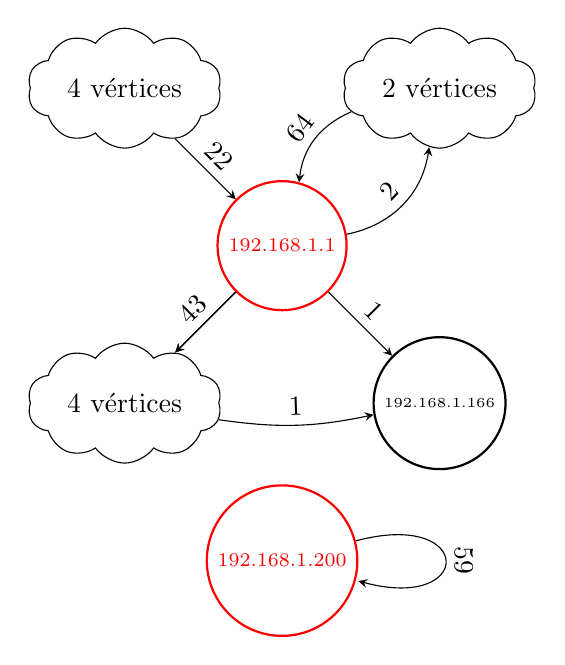
\begin{tikzpicture}
    \tikzset{vertex/.style = {shape=circle,draw,thick,minimum size=2em,font=\tiny}}
    \tikzset{NoDistinguido/.style = {shape=circle,draw,thick,minimum size=2em,font=\tiny}}
    \tikzset{Distinguido/.style = {shape=circle,draw,red,thick,minimum size=2em,font=\scriptsize}}


    \tikzset{myCloud/.style = {shape=cloud,draw, cloud puffs=10,cloud puff arc=110, aspect=2, inner ysep=0.5em}}

    \tikzset{flecha/.style = {->,>=stealth,sloped,auto=false}}

    \node[myCloud] (NubeA) at (-2,2) {4 vértices};
    \node[myCloud] (NubeC) at (2,2) {2 vértices};
    \node[myCloud] (NubeB) at (-2,-2){4 vértices};

    \node[Distinguido] (node1) at (0,0) {192.168.1.1};
    \node[NoDistinguido] (node166) at (2,-2) {192.168.1.166};
    \node[Distinguido] (node200) at (0,-4) {192.168.1.200};

    \draw [flecha] (NubeA) to node[above] {22} (node1);

    \draw[flecha] (node1) edge [bend right=35] node[above] {2} (NubeC);
    \draw[flecha] (NubeC) edge [bend right=30] node[above] {64} (node1);


    \draw[flecha] (node1) edge node[above] {43} (NubeB);

    \draw[flecha] (NubeB) edge [bend right=10] node[above] {1} (node166);
    \draw[flecha] (node1) edge node[above] {1} (node166);

    \path[->,flecha] (node200)
            edge [loop right=30] node [above] {59} ();

    \draw[flecha] (node1) edge (NubeB);

\end{tikzpicture}

	\label{grafo_cafe}
\end{figure}

\begin{figure}[H]
  \begin{center}
    \includegraphics[scale = 0.5]{img/Cafe-information-S1.pdf}
    \caption{Información de los simbolos de la fuente S1 para Cafe}
    \label{informacion_cafe}
  \end{center}
\end{figure}

La cantidad de nodos identificados en total es razonable para un café, pero en base a nuestro conocimiento de la red tiene sentido sospechar que existían nodos que no fueron divisados, considerando la cantidad de personas y empleados que se encontraban en el lugar en el momento. El número de vértices del grafo, que muestra 5 nodos más que no aparecieron como símbolos de la fuente, se acerca más a un valor esperable.

El método utilizado para definir símbolos distinguidos señaló dos vértices en la figura \ref{grafo_cafe}. De ellos uno, el 192.168.1.1, respeta la convención de direcciones utilizada para \textit{routers} o \textit{default gateways}. El grafo construido refleja que su vértice en el mismo puede asociarse a un router en base a su patrón de relaciones topológicamente central en la red de tráfico ARP. Esto se corresponde con el conocimiento acerca de la red de que efectivamente existe de un router con salida a internet.

Por otro lado, el segundo símbolo señalado corresponde a un vértice con un comportamiento anómalo a priori. Entre sus posibles justificaciones se encuentra una estrategia estándar discutida en el RFC 5227 \footnote{IPv4 Address Conflict Detection https://tools.ietf.org/html/rfc5227} para prevenir conflictos de IP. También es utilizado para permitir a otros vértices como el \textit{router} actualizar sus tablas ARP para luego comunicarse con él.

En conclusión, en lo que respecta la distinción de un default gateway, podemos ver que fue parcialmente exitoso al identificar al router pero dar un falso positivo que es el 192.168.1.200. Notamos de todas maneras a favor del criterio de distinción que el que efectivamente se trata del router tiene la menor información entre los dos según la figura \ref{informacion_cafe}.

Se tiene conocimiento de la presencia de cámaras IPs conectadas a la red, las cuales en este caso puede corresponder a los dos vértices agrupados que intercambian un gran número de paquetes con el aparte \textit{router}.

Es interesante notar que para esta red de haber utilizado el origen en lugar del destino de los paquetes para símbolos hubiera incluido estos dos entre sus resultados.

%%%%%%%%%%%%%%%%%%%%%

\subsection{\textbf{CoinFactory}}

\subsubsection{Fuente $S$}

\begin{center}\small
	\begin{tabular}{ c | c | c }
	  $I(\SimbBroadcast)$ & $I(\SimbUnicast)$ & $H(S)$ \\
	  \hline
	  4.54 & 0.06 & 0.0256 \\
	\end{tabular}
\end{center}

La entropía de la fuente es 50 veces más chica que la máxima.
Al igual que el caso anterior la cantidad de paquetes \textit{broadcast} representa un porcentaje chico del total, de lo se puede intuir de manera similar al experimento anterior que los protocolos de control de la red generaron un \textit{overhead} poco significativo.

\medskip

\subsubsection{Fuente $S_1$}

\begin{center}\small
	\begin{tabular}{ c | c }
	  $|nodos|$ & $|distinguidos|$ \\
	  \hline
	  15 & 1 \\
	\end{tabular}
\end{center}

\begin{figure}[H]
	\centering
	\caption{CoinFactory}
	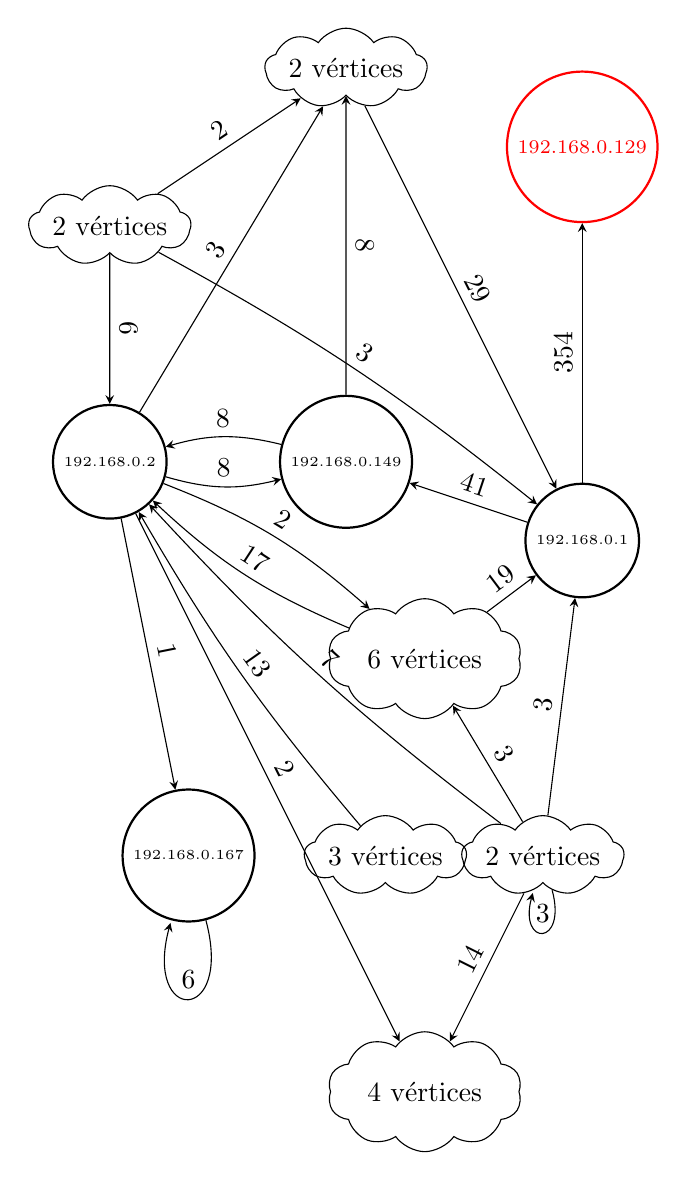
\begin{tikzpicture}

    \tikzset{vertex/.style = {shape=circle,draw,thick,minimum size=2em,font=\tiny}}
    \tikzset{NoDistinguido/.style = {shape=circle,draw,thick,minimum size=2em,font=\tiny}}
    \tikzset{Distinguido/.style = {shape=circle,draw,red,thick,minimum size=2em,font=\scriptsize}}
    \tikzset{myCloud/.style = {shape=cloud,draw, cloud puffs=10,cloud puff arc=110, aspect=2, inner ysep=0.5em}}

    \tikzset{myCloudSmaller/.style = {shape=cloud,draw, cloud puffs=9,cloud puff arc=110, aspect=3, inner ysep=0em, inner xsep=0em}}
    \tikzset{flecha/.style = {->,>=stealth,sloped,auto=false}}

    \node [NoDistinguido] (router1) at (3,0) {192.168.0.1};
    \node [Distinguido] (nodo129) at (3,5) {192.168.0.129};
    \draw [flecha] (router1)
        to node[above] {354} (nodo129);


    \node [NoDistinguido] (router2) at (-3,1) {192.168.0.2};


    %IPs 173, 163
    \node [myCloudSmaller] (NubeE) at (0,6) {2 vértices};
    \draw [flecha] (router2)
        to node[above] {3} (NubeE);
    \draw [flecha] (NubeE)
        to node[above] {29} (router1);


    %IPS 114, 118,  121, 122,  123, 145, 164, 178
    \node [myCloud] (NubeA) at (1,-1.5) {6 vértices};
    \draw [flecha] (NubeA)
        to node[above] {19} (router1);
    \draw [flecha] (NubeA)
        to [bend left=10] node[above] {17} (router2);
    \draw [flecha] (router2)
        to [bend left=10] node[above] {2} (NubeA);


    %IPs 177, 153 y 168
    \node [myCloudSmaller] (NubeB) at (0.5,-4) {3 vértices};
    \draw [flecha] (NubeB)
            to[bend left=5] node[above] {13} (router2);


    \node [myCloudSmaller] (NubeF) at (2.5,-4) {2 vértices};
    \draw [flecha] (NubeF)
         to node[above] {3} (router1);
    \draw [flecha] (NubeF)
         to[bend left=5] node[above] {7} (router2);
    \draw [flecha] (NubeF)
        to node[above] {3} (NubeA);
    \path[->,flecha] (NubeF)
            edge [loop below] node [above] {3} ();


    %IPs 102, 116, 139 y 154
    \node [myCloud] (NubeC) at (1,-7) {4 vértices};
    \draw [flecha] (router2)
        to node[above] {2} (NubeC);
    \draw [flecha] (NubeF)
        to node[above] {14} (NubeC);


    %IPs 109, 137
    \node[myCloudSmaller] (NubeD) at (-3,4) {2 vértices};
    \draw [flecha] (NubeD)
        to [bend left=5] node[above] {3} (router1);
    \draw [flecha] (NubeD)
        to node[above] {6} (router2);
    \draw [flecha] (NubeD)
        to node[above] {2} (NubeE);


    \node [NoDistinguido] (nodo149) at (0,1) {192.168.0.149};
    \draw [flecha] (nodo149)
        to node[above] {8} (NubeE);
    \draw [flecha] (nodo149)
        to [bend right=15]  node[above] {8} (router2);
    \draw [flecha] (router2)
        to [bend right=15]  node[above] {8} (nodo149);
    \draw [flecha] (router1)
        to node[above] {41} (nodo149);


    \node [NoDistinguido] (nodo167) at (-2,-4) {192.168.0.167};
    \draw [flecha] (router2)
        to node[above] {1} (nodo167);
    \path[->,flecha] (nodo167)
            edge [loop below] node [above] {6} ();

\end{tikzpicture}

\end{figure}

\begin{figure}[H]
  \begin{center}
    \includegraphics[scale = 0.5]{img/Pyme-information-S1.pdf}
    \caption{Información de los simbolos de la fuente S1 para CoinFactory}
    \label{informacion_pyme}
  \end{center}
\end{figure}

El grafo generado a través de los paquetes capturados refleja dos vértices, de IPs 192.168.0.1 y 192.168.0.2, con un comportamiento que se presume propio de un \textit{router} o un \textit{default gateway} al tener direcciones físicas muy solicitadas por muchos nodos distintos. Esto se corresponde en parte con el conocimiento acerca de la red según el cual existe al menos un router con salida a internet. En este caso, el método de detección de nodos distinguidos no los marcó como tales, y en su lugar señaló un vértice, el 192.168.0.129, que recibió una cantidad de pedidos \textit{who-has} anómala respecto a los demás. Nuevamente dio un falso positivo, pero además tampoco distinguió al que sospechamos que es el router. Sin embargo, notamos que los siguientes dos nodos con menor información son los nodos .1 y .2 según el gráfico en la figura \ref{informacion_pyme}, de modo que en este caso también observamos una correlación entre el rol de \textit{default gateway} y el proveer poca información en el modelo de fuente $S_1$.

Se puede ver en el grafo que los pedidos fueron generados en su enteridad por un solo nodo, específicamente uno de los que sospechamos que es un router, por lo que el comportamiento aparentemente anómalo estaría asociado a él. Sabemos que, según el RFC citado del protocolo, cualquier nodo en la red que tenga en su tabla ARP una entrada para el .1 la actualizará al ver cada uno de los pedidos. Suponiendo la preexistencia de dichas entradas en las tablas de los hosts de la red (generada en una instancia previa a la captura), si bien genera una cantidad relativamente alta de broadcasts que cargan al medio físico y a todos los hosts de la red, este tipo de política puede reducir la necesidad del resto de los hosts de consultar por la dirección física del sospechado router, centralizando en él la responsabilidad de ``informar'' su dirección. Se sabe que la red corresponde a una empresa, por lo que se espera la presencia de servicios como impresoras red, servidores web, servidores DNS etc. Entre los argumentos que pueden justificar este comportamiento también se encuentra la posibilidad de que el nodo receptor de estos pedidos sea host de un servicio de ese tipo. Otra posibilidad es la existencia de configuraciones que requieran la resolución periódica de la dirección física de esa IP de manera \textit{ad-hoc}. Un caso de esto puede ocurrir al tener un dispositivo vinculado con una IP en la lista de clientes DHCP del \textit{router}, con un \textit{lease time} arbitrariamente grande que se apagó.

Otro comportamiento particular observado es el del nodo .167, que envía seis \textit{gratuitous ARP requests}. Al igual que en el experimento anterior, esto puede asociarse con la aplicación de un protocolo de detección de conflictos de direcciones IP.

En este caso, de haber utilizado el origen en lugar de los destinos de los \textit{who-has}, el método de obtención de símbolos distinguidos probablemente hubiera marcado al vértice con IPs \texttt{192.168.0.1} como tal. Además, hubiera detectado como hosts a 9 de los que se encuentran entre los nodos agrupados del grafo y que resultaron como falsos negativos, ya que en el grafo se observan 24 nodos y $S_1$ arrojó 15 símbolos distintos durante la captura.

%%%%%%%%%%%%%%%%%%%%%

\subsection{\textbf{ComercioLibre}}

\subsubsection{Fuente $S$}

\begin{center}\small
	\begin{tabular}{ c | c | c }
	  $I(\SimbBroadcast)$ & $I(\SimbUnicast)$ & $H(S)$ \\
	  \hline
	  5.13 & 0.04 & 0.187 \\
	\end{tabular}
\end{center}

Al igual que antes se puede observar que la entropía no es máxima. En este caso el tráfico de los paquetes \textit{unicast} representa el 97\% del total, lo cual induciría una conclusión similar a la de los experimentos anteriores respecto del \textit{overhead} producido por mensajes \textit{broadcast} de control.

\medskip

\subsubsection{Fuente $S_1$}

\begin{center}\small
	\begin{tabular}{ c | c }
	  $|nodos|$ & $|distinguidos|$ \\
	  \hline
	 15 & 2 \\
	\end{tabular}
\end{center}

\begin{figure}[H]
	\centering
	\caption{ComercioLibre}
	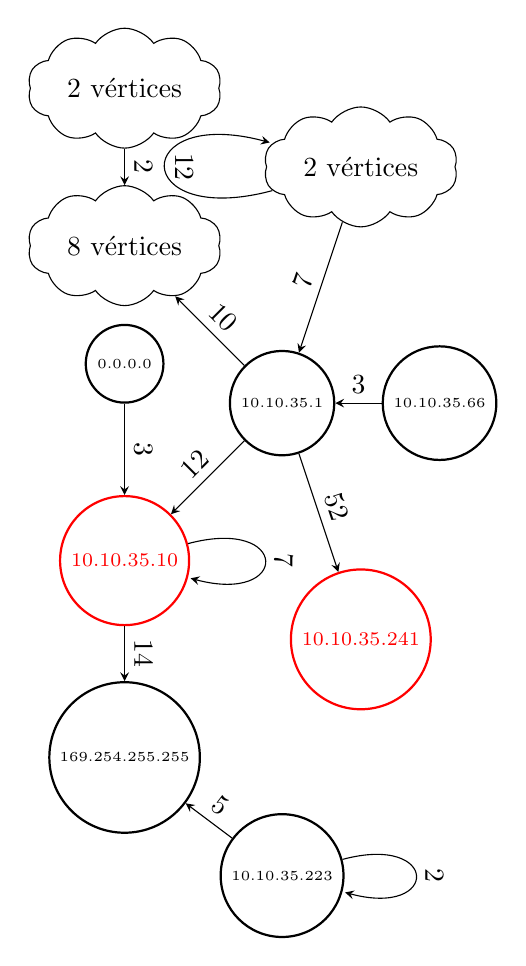
\begin{tikzpicture}
    \tikzset{NoDistinguido/.style = {shape=circle,draw,thick,minimum size=2em,font=\tiny}}
    \tikzset{Distinguido/.style = {shape=circle,draw,red,thick,minimum size=2em,font=\scriptsize}}
    \tikzset{myCloud/.style = {shape=cloud,draw, cloud puffs=10,cloud puff arc=110, aspect=2, inner ysep=0.5em}}

    \tikzset{flecha/.style = {->,>=stealth,black,sloped,auto=false}}

    \node[myCloud] (NubeA) at (-2,2) {8 vértices};
    \node[myCloud] (NubeB) at (-2,4) {2 vértices};

    \node[myCloud] (NubeC) at (1,3) {2 vértices};

    \node[NoDistinguido] (aparenteRouter) at (0,0) {10.10.35.1};
    \node[NoDistinguido] (node66) at (2,0) {10.10.35.66};


    \node[NoDistinguido] (node0) at (-2,0.5) {0.0.0.0};
    \node[Distinguido] (dist1) at (-2,-2) {10.10.35.10};
    \node[NoDistinguido] (node255) at (-2,-4.5) {169.254.255.255};
    \node[NoDistinguido] (node223) at (0,-6) {10.10.35.223};

    \node[Distinguido] (dist2) at (1,-3) {10.10.35.241};


    %Entradas a la nubeA
    \draw [flecha] (aparenteRouter) to node[above] {10} (NubeA);
    \draw [flecha] (NubeB) to node[above] {2} (NubeA);

    %Aparente router a vértices Distinguidos
    \draw [flecha] (aparenteRouter) to node[above] {12} (dist1);
    \draw [flecha] (aparenteRouter) to node[above] {52} (dist2);

    %Un colgado
    \draw [flecha] (node66) to node[above] {3} (aparenteRouter);

    %

    \draw [flecha] (node0) to node[above] {3} (dist1);

    \draw [flecha] (dist1) to node[above] {14} (node255);
    \path[flecha] (dist1)
            edge [loop right=30] node [above] {7} ();

    \draw [flecha] (node223) to node[above] {5} (node255);
    \path[flecha] (node223)
            edge [loop right=30] node [above] {2} ();


    \draw [flecha] (NubeC) to node[above] {7} (aparenteRouter);
    \path[flecha] (NubeC)
            edge [loop left] node [above] {12} ();

%\iffalse
%Dejo esto por si quieren partir la Nube C
%    \node[NoDistinguido] (node37) at (0,2) {10.10.35.37};
%    \node[NoDistinguido] (node141) at (2,2) {10.10.35.141};
%    \draw [flecha] (node37) to node[above] {3} (aparenteRouter);
%    \path[flecha] (node37)
%            edge [loop above] node [above] {6} ();
%
%    \draw [flecha] (node141) to node[above] {4} (aparenteRouter);
%    \path[flecha] (node141)
%            edge [loop right=30] node [above] {6} ();
%\fi

\end{tikzpicture}

    \label{grafo_ecommerce}
\end{figure}

\begin{figure}[H]
  \begin{center}
    \includegraphics[scale = 0.5]{img/ECommerce-information-S1.pdf}
    \caption{Información de los simbolos de la fuente S1 para ComercioLibre}
    \label{informacion_ecommerce}
  \end{center}
\end{figure}

La fuente $S_1$ para este experimento emitió un total de 15 símbolos distintos. Dos de estos, 10.10.35.10 y 10.10.35.241 fueron señalados como distinguidos. Con un análisis análogo a la de los experimentos anteriores, conociendo que en este caso también se trata de una red con salida a internet, podemos sospechar que el 10.10.35.1 es en realidad el router, y que los marcados distinguidos no lo son, obteniendo en este experimento dos falsos positivos por parte del criterio de distinción. Se desconoce a qué dispositivos correspondían, pero dado que se trata de una red empresarial, podríamos atribuir lo altamente solicitadas que parecen ser sus direcciones físicas a que sean hosts de servicios como repetidores, impresoras o servidores. De modo similar a los experimentos anteriores, nos encontramos con que el sospechado router es el siguiente con menor información luego del host de IP 169.254.255.255 que, como veremos a continuación, no representa un verdadero host en la red.

Se da una situación parecida a la mencionada en el experimento anterior, en la que el candidato a ser router pregunta una cantidad relativamente alta de veces por la dirección física del .24. Esto refuerza la noción de que podría corresponder a un nodo con algún servicio especial.

En la figura \ref{grafo_ecommerce} se pueden observar dos IPs que no pertenecen a lo que parece ser una subred de direcciones 10.10.35.X. Por un lado, la \texttt{0.0.0.0}, no pertenece al conjunto de símbolos emitidos por la fuente ya que no fue receptor de ningún paquete \textit{who-has}. En principio, esto podría clasificarse como un falso negativo, es decir, un host que nuestro modelo de la red como fuente se perdió por tomar sólo las direcciones de destino. Sin embargo, esto no tendría sentido por el claro hecho de que la dirección ni siquiera tiene sentido como perteneciente a la red. Observando que la misma generó 3 ARP \textit{request} con IP destino 10.10.35.10, podemos hacer alusión al citado RFC 5227 \footnote{sección: 2.1.1. Probe Details} donde se explica que este comportamiento es generado para evitar un conflicto de IPs. El host en cuestión envía tres pedidos \textit{who-has} con la IP que quiere comenzar a usar como destino completando el campo de \textit{origen} con la IP \texttt{0.0.0.0}, que es una dirección reservada para usos como este según el RFC 5735\footnote{https://tools.ietf.org/html/rfc5735}, para no alterar las tablas ARP de otros \textit{hosts} en caso que ya se este utilizando la IP. Si no recibe respuesta se asigna esa IP y la anuncia. Los dos envíos de \textit{who-has} por parte del .223 a sí mismo pueden ser asociados al RFC 5227 también.

Por otro lado, la IP \texttt{169.254.255.255} fue un símbolo emitido por $S_1$ y se trata de una dirección reservada según el RFC 5735 para uso local, comúnmente relacionado al protocolo DHCP.

Notemos además la discrepancia entre la cantidad de nodos detectada por la fuente de 15 con la que existe en el grafo de 17 si se ignoran las IPs especiales mencionadas antes.

%%%%%%%%%%%%%%%%%%%%%

\subsection{\textbf{Cumpleaños}}

\begin{center}\small
	\begin{tabular}{ c | c | c }
	  $I(\SimbBroadcast)$ & $I(\SimbUnicast)$ & $H(S)$ \\
	  \hline
	  0.53 & 1.68 & 0.894 \\
	\end{tabular}
\end{center}

La red analizada para este experimento presentó un comportamiento distinto a las anteriores. La entropía se acercó mucho más al máximo, y el en este caso fueron más los paquetes \textit{broadcast} que los \textit{unicast}, alcanzando un 68\% del total. Esto sugiere un comportamiento anómalo ya que la proporción de envíos \textit{broadcast} sí parece suponer un \textit{overhead} muy alto en la red, mientras que lo esperable es que la mayoría del tráfico en una red hogareña con conexión a internet sea con paquetes \textit{unicast} utilizados para transmitir datos, tal como sucedió en las redes anteriores.

\subsubsection{Fuente $S_1$}

\begin{center}\small
	\begin{tabular}{ c | c }
	  $|nodos|$ & $|distinguidos|$ \\
	  \hline
	  253 & 177 \\
	\end{tabular}
\end{center}

\begin{figure}[H]
	\centering
	\caption{Cumpleaños}
	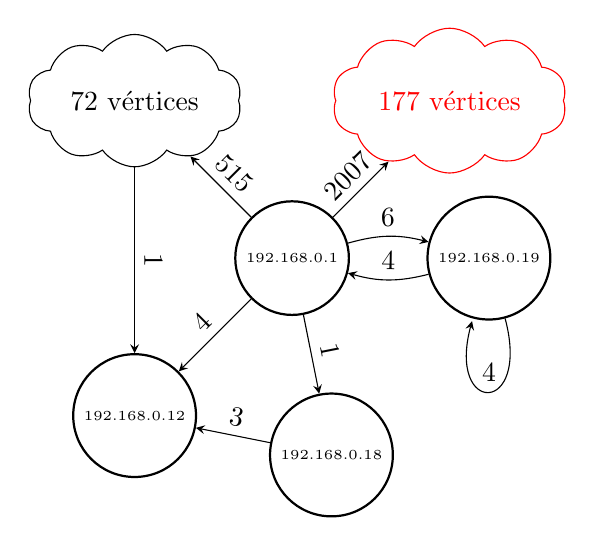
\begin{tikzpicture}
    \tikzset{vertex/.style = {shape=circle,draw,thick,minimum size=2em,font=\tiny}}
    \tikzset{NoDistinguido/.style = {shape=circle,draw,thick,minimum size=2em,font=\tiny}}
    \tikzset{Distinguido/.style = {shape=circle,draw,red,thick,minimum size=2em,font=\scriptsize}}

    \tikzset{myCloud/.style = {shape=cloud,draw, cloud puffs=10,cloud puff arc=110, aspect=2, inner ysep=0.5em}}

    \tikzset{flecha/.style = {->,>=stealth,sloped,auto=false}}

    \node[myCloud,red] (NubeA) at (2,2) {177 vértices};

    \node[myCloud] (NubeB) at (-2,2) {72 vértices};

    \node[NoDistinguido] (router1) at (0,0) {192.168.0.1};
    \node[NoDistinguido] (nodo12) at (-2,-2) {192.168.0.12};
    \node[NoDistinguido] (nodo18) at (0.5,-2.5) {192.168.0.18};
    \node[NoDistinguido] (nodo19) at (2.5,0) {192.168.0.19};

    \draw [flecha] (router1) to node[above] {515} (NubeB);
    \draw [flecha] (router1) to node[above] {2007} (NubeA);

    \draw [flecha] (router1) to node[above] {4} (nodo12);
    \draw [flecha] (NubeB) to node[above] {1} (nodo12);
    \draw [flecha] (router1) to node[above] {1} (nodo18);
    \draw [flecha] (nodo18) to node[above] {3} (nodo12);
    \draw [flecha] (router1) [bend left=15] to node[above] {6} (nodo19);
    \draw [flecha] (nodo19) to[bend left=15] node[above] {4} (router1);

    \path[->,flecha] (nodo19)
            edge [loop below] node [above] {4} ();
\end{tikzpicture}

    \label{grafo_cumple}
\end{figure}

\begin{figure}[H]
  \begin{center}
    \includegraphics[scale = 0.5]{img/Cumple-information-S1.pdf}
    \caption{Información de los simbolos de la fuente S1 para Cumpleaños}
    \label{informacion_cumple}
  \end{center}
\end{figure}

El tráfico ARP resultó muy alto. Se capturaron en total 2545 mensajes ARP sobre un total de 3812 capturados. La fuente $S_1$ generó en total 253 símbolos y más de dos tercios de esos fueron distinguidos, lo que indica que hubo pocos símbolos con mucha información. Se sabe que al momento de la captura se encontraban aproximadamente 20 potenciales usuarios presentes en el ámbito físico, con lo cual el número detectado de hosts está lejos de poder ser real. Naturalmente, tampoco tiene sentido pensar en un dominio de broadcast con 177 routers. Sabiendo que al menos uno existía al saber que se trató de una red hogareña con un router con salida a internet, que se considera que debe de ser el 192.168.0.1, ya podemos concluir que el criterio de distinción no sirvió en este caso para identificar al \textit{default gateway}.

En la figura \ref{informacion_cumple} están representados los 15 símbolos con más y menos información. La línea punteada refleja la presencia de un intervalo de símbolos no representados para una mejor visualización. En el grafo \ref{grafo_cumple} se puede observar de forma más clara la presencia de los nodos omitidos del gráfico.

El que suponemos \textit{default gateway} envió 2007 paquetes ARP con destino a 177 \textit{host} distintos, dando como alrededor de 11 paquetes por cada IP de esa nube del grafo. También envió otros 515 paquetes a otro grupo de IPs, promediando los 7 paquetes por dirección. La nubes que se ven fueron agrupadas de acuerdo a estos valores. Hay evidencia suficiente para decir que un \textit{host} realizó un comportamiento de barrido sobre casi todo el rango de direcciones IP pertenecientes a la red \texttt{192.168.1.0/24} enviando paquetes ARP \textit{request} con la IP del \textit{default gateway} como dirección origen a cada una varias veces. Una posible explicación para este comportamiento es que algún \textit{host}, que a priori parece ser el router en este caso, está realizando consultas ARP periódicas para detectar que direcciones IP están en uso en la red.

Notemos por último que, al igual a lo sucedido con en casos anteriores, haber utilizado la dirección origen de los mensajes \textit{who-has} en lugar del destino seguramente hubiera señalado este símbolo.

%%%%%%%%%%%%%%%%%%%%%

% \section{\textbf{Figuras}}

%Conclusiones
\section{Conclusiones}

Salvando el caso del experimento \textit{Cumpleaños}, las redes presentan un comportamiento parecido respecto de la proporción de mensajes de control en el tráfico de la red. Si bien no tenemos valores de referencia contra los que comparar, al tener tres redes con proporciones parecidas de mensajes \textit{broadcast} en contraste con los \textit{unicast} tenemos un buen indicio inicial de qué \textit{overhead} puede esperarse por parte de protocolos de control.

En cuando a la distinción de hosts en la red, vemos que en todos los casos nuestra definición de $S_1$ llevó a falsos negativos que, más aún, serían detectados de haber elegido las IPs de origen de los mensajes \textit{who-has}. En cambio, no hay evidencia de falsos positivos, salvo en el caso del barrido lineal en \textit{Cumpleaños}.

El criterio planteado de identificación de nodos distinguidos en base a la información y entropía en ningún caso dio el mejor resultado, que sería el de identificar únicamente al \textit{default gateway}; en todos los casos dio falsos positivos, y sólo en uno hay evidencia para suponer que lo detectó correctamente. Esto, en gran parte, se debe a comportamientos inesperados de algunos hosts. Por otra, puede atribuirse a que ocurre más seguido de lo que esperábamos que un router sea \textit{emisor} de mensajes \textit{who-has}, hecho que, como señalamos en la sección anterior, significa que hubiéramos tenido mejores resultados de identificación de \textit{default gateways} de haber elegido que los símbolos de $S_1$ sean IPs de origen.

Si bien nuestros datos no reflejan una clara relación entre la entropía y la cantidad de nodos, sí pensamos que el cálculo de la entropía y la cantidad de información provista por los hosts puede ser un dato útil a la hora de formular un criterio para clasificarlos, idea respaldada por la teoría, por la identificación parcialmente exitosa en el experimento \textit{Café} y por el haber clasificado a los routers entre los hosts de menor información en nuestros resultados.

Podemos agregar como conclusión general que, por la variedad de protocolos que existen, la naturaleza descentralizada de las redes, la pluralidad de tecnologías que se encuentran en ellas y lo heterogéneas que por lo tanto suelen resultar, desarrollar herramientas simples para estudiarlas de manera general y automática es una tarea muy difícil. La misma variabilidad de los sistemas que serían objeto de estudio de dichas herramientas hace que se requiera mínimamente también una variedad amplia de criterios para su evaluación. Como trabajo futuro, nos plantearíamos como alternativa realizar experimentos utilizando la misma herramienta presentada en este trabajo en ambientes más controlados, corriéndola sobre redes de las que se conocen características de infraestructura a un grado un poco mayor. Otra alternativa es seguir experimentando en sistemas pocos controlados para derivar criterios más precisos. Un primer candidato que tendría buen potencial en base a nuestros datos es uno que complemente el modelado de la red como una fuente $S_1$ con símbolos definidos tanto en base a direcciones de destino como de origen.


\appendices


\iffalse
%%Dejo esto por si queremos hacer referencias a documentación de Scapy
\begin{thebibliography}{1}
\bibitem{IEEEhowto:kopka}
H.~Kopka and P.~W. Daly, \emph{A Guide to \LaTeX}, 3rd~ed.\hskip 1em plus
  0.5em minus 0.4em\relax Harlow, England: Addison-Wesley, 1999.
\end{thebibliography}
\fi

\end{document}